\chapter{Design and Architecture of the Solution}
\label{chap:design}

\section*{Introduction}

This chapter presents the design that satisfies the requirements of
Chapter~\ref{chap:requirements}. It describes the platform as a whole: its
architectural objectives, its logical decomposition, its runtime and deployment
model, its security and trust boundaries, its persistence, and its simulation
workflow. It then details the governed multi-agent layer, agent by agent, and the
observability and operational architecture around it. The result-interpretation
agent, the visualization layer, and the evaluation harness, the components at the
heart of the report's central question, are presented in this same flow and given
deeper treatment, always as parts of the complete system rather than in
isolation.

The design is guided by one central constraint: the deterministic optimizer
remains the authority for operational and financial results. Every other
subsystem exists to make that authority easier to access, safer to operate, and
more efficient to use. A structural theme follows from this constraint and recurs
throughout the chapter: the platform keeps interactive coordination on the request
path separate from \textbf{two durable, asynchronous execution planes} off it, one
for deterministic simulation and one for agent reasoning. Heavy or probabilistic
work therefore never blocks the interface, each plane is dispatched durably and
recovered on its own, and neither can seize numerical authority.

\section{Architectural objectives and system role}
\label{sec:arch-objectives}

The design starts from the limitations identified earlier and translates them into
architectural objectives. Table~\ref{tab:objectives} states each objective and its
architectural implication.

\begin{table}[H]
  \centering
  \begin{tabularx}{\linewidth}{@{}
      >{\raggedright\arraybackslash}p{4.3cm}
      >{\raggedright\arraybackslash}X @{}}
    \toprule
    \textbf{Objective} & \textbf{Architectural implication} \\
    \midrule
    Preserve numerical authority & Keep optimization in the deterministic core;
      route assisted work toward validated inputs and approved actions rather than
      model-generated results. \\
    \addlinespace
    Support long-running computation & Separate interactive traffic from
      simulation through asynchronous dispatch, persisted job state, and
      independently managed compute. \\
    \addlinespace
    Protect enterprise access & Move identity enforcement to the platform edge
      through federated authentication, avoiding application-owned identity
      complexity. \\
    \addlinespace
    Improve maintainability & Give each concern (interaction, coordination,
      computation, persistence, assistance, platform) a clear owner. \\
    \addlinespace
    Make deployments repeatable & Treat infrastructure, runtime configuration, and
      releases as versioned delivery artifacts. \\
    \addlinespace
    Govern language-model assistance & Typed tool contracts, observable
      interactions, validation, and human approval before any mutation. \\
    \bottomrule
  \end{tabularx}
  \caption{Architectural objectives and their implications.}
  \label{tab:objectives}
\end{table}

The architecture is therefore not a single tooling choice but a set of
\textbf{boundaries}: between users and protected services, between synchronous
requests and asynchronous computation, between authoritative computation and
probabilistic assistance, and between product logic and operating-environment
concerns.

\section{Logical decomposition}
\label{sec:logical}

At the highest level the system is organized as a progression from interaction to
computation (Figure~\ref{fig:logical-layers}). Users work through a
\textbf{presentation layer}; a
\textbf{coordination layer} validates requests and coordinates state transitions;
long-running optimization is delegated to dedicated \textbf{execution} capacity;
durable stores hold canonical state and large artifacts; the \textbf{agentic
layer} assists through bounded proposals; and the \textbf{platform layer} provides
the secure operating envelope.

\begin{figure}[H]
  \centering
  \resizebox{0.9\linewidth}{!}{%
  \begin{tikzpicture}[
    font=\small,
    box/.style={rectangle, rounded corners=3pt, draw=black!55, thick,
      align=center, inner sep=5pt, fill=white, minimum height=0.8cm, text width=3.2cm},
    core/.style={rectangle, rounded corners=4pt, draw=teal!70!black, line width=1pt,
      align=center, inner sep=5pt, fill=teal!8, minimum height=0.8cm, text width=3.2cm},
    arr/.style={-{Stealth[length=2.5mm]}, line width=0.9pt, black!65},
    darr/.style={-{Stealth[length=2.5mm]}, line width=0.9pt, black!55, dashed},
  ]
    \node[box, text width=1.4cm] (user) {User};
    \node[box, below=0.7cm of user] (pres) {Presentation layer};
    \node[box, below=0.9cm of pres] (coordn) {Coordination layer\\(typed contracts)};
    \node[box, right=2.4cm of coordn] (agent) {Agentic layer\\(bounded proposals)};
    \node[core, below left=0.9cm and -1.4cm of coordn] (exec) {Deterministic execution};
    \node[box, below right=0.9cm and -1.4cm of coordn] (pers) {Persistence\\(state and artifacts)};
    \draw[arr] (user) -- (pres);
    \draw[arr] (pres) -- node[left, font=\footnotesize, black!60]
      {authenticated requests} (coordn);
    \draw[arr] (coordn) -- (exec);
    \draw[arr] (coordn) -- (pers);
    \draw[arr] (exec) -- (pers);
    \draw[arr] (coordn.15) -- node[above, font=\footnotesize, black!60]
      {assisted turns} (agent.165);
    \draw[darr] (agent.195) -- node[below, font=\footnotesize, black!60]
      {typed proposals} (coordn.345);
    \begin{scope}[on background layer]
      \node[rectangle, rounded corners=5pt, draw=black!25, fill=black!4,
        inner sep=10pt, fit=(coordn)(agent)(exec)(pers),
        label={[font=\footnotesize\bfseries, black!50]below:Platform layer
          (secure operating envelope)}] {};
    \end{scope}
  \end{tikzpicture}%
  }
  \caption{Logical decomposition: authority flows from the coordination layer to
    the deterministic core, while the agentic layer may only propose.}
  \label{fig:logical-layers}
\end{figure}

The important point is the direction of authority. User-facing and agentic
components may prepare, explain, and request changes, but state transitions pass
through the coordination layer, and numerical outputs pass through the
deterministic engine. This avoids two weak designs: exposing the solver directly
(forcing users to understand its internals) and hiding the solver behind an
autonomous conversational layer (weakening reproducibility and auditability).

\subsection{System graph views}

A useful way to reason about the architecture is to view it as a set of directed
graphs, each with its own nodes and its own authority rule
(Table~\ref{tab:graphs}). This makes explicit which component may transform state
and which may only request or observe it.

\begin{table}[H]
  \centering
  \begin{tabularx}{\linewidth}{@{}
      >{\raggedright\arraybackslash}p{3.1cm}
      >{\raggedright\arraybackslash}X @{}}
    \toprule
    \textbf{Graph} & \textbf{Nodes and authority rule} \\
    \midrule
    Runtime execution & Presentation, access boundary, coordination, asynchronous
      execution, persistence, observability. Interactive requests, simulation
      jobs, and observability events follow different edges; long-running
      optimization never blocks the request path. \\
    \addlinespace
    Domain topology & Project canvas, asset and market nodes, flow edges, scenario
      parameters. The user edits an application-level graph; the coordination
      layer validates it before it becomes an optimization input. \\
    \addlinespace
    Simulation & Submitted scenario, persisted input, dispatched job, deterministic
      execution, output artifacts. Heavy payloads move by reference, while the
      dispatch path carries identifiers and execution intent. \\
    \addlinespace
    Assisted action & User intent, Director, specialist reasoning, typed proposal,
      validation, approval, committed mutation. Model output may propose, but only
      validated and approved proposals mutate project state. \\
    \bottomrule
  \end{tabularx}
  \caption{System graph views and their authority rules.}
  \label{tab:graphs}
\end{table}

\section{Runtime and deployment architecture}
\label{sec:runtime}

The runtime separates interactive work on the request path from the two
asynchronous execution planes introduced above (Figure~\ref{fig:two-planes}). A
normal request enters through the presentation layer, crosses the authenticated
edge, and reaches the coordination layer, which either reads or updates project
state, serves assisted interactions, or dispatches work to one of the two planes.
The first runs \textbf{deterministic simulation}, described here; the second runs
the \textbf{agent reasoning system}, described in
Section~\ref{sec:agent-runtime}. Because a grid search can
launch thousands of hour-by-hour simulations and run far longer than a web request
should block for, simulation work is placed on an \textbf{asynchronous execution
path}: the backend enqueues a job on a dedicated queue, a separate pool of workers
consumes it, runs the deterministic engine, and persists the outputs for later
retrieval, while the interface stays responsive and polls for status.

This split is essential because it lets execution capacity scale independently of
interactive capacity: heavy workloads are absorbed by adding workers, so the
interactive experience stays responsive under load rather than competing with
computation for capacity. Scaling follows the same
separation, with backlog depth as the signal that drives additional execution
capacity, while the coordination side is scaled more conservatively so that
capacity improvements never compromise the correctness of conversational
checkpoint state.

\begin{figure}[H]
  \centering
  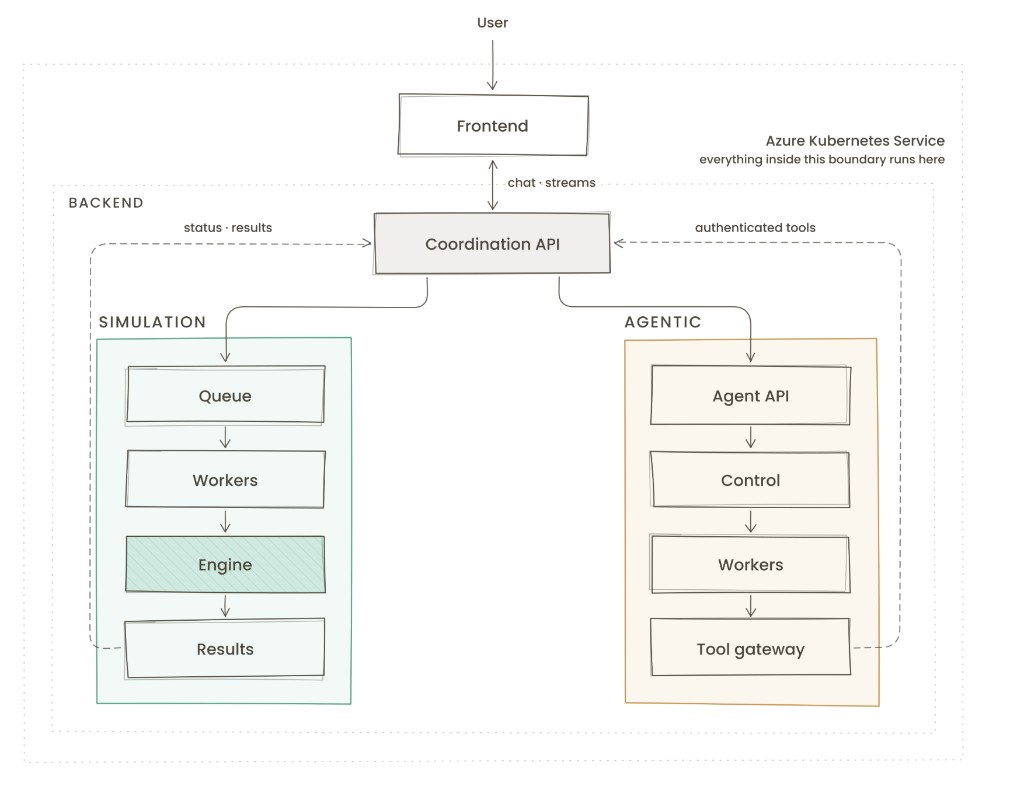
\includegraphics[width=0.9\linewidth]{Figures/runtime_planes.png}
  \caption{The application on Azure Kubernetes Service: the backend and the two
    durable execution planes, simulation and agentic, with their controlled
    return paths.}
  \label{fig:two-planes}
\end{figure}

\subsection{Cloud and deployment model}

The platform runs in a managed cloud environment rather than on manually operated
servers. The environment is separated into foundational resources (build, naming,
shared storage), infrastructure resources (private networking, controlled
administration, compute capacity, cost controls), and runtime support services
(access control, authentication support, observability, and operational
monitoring). Access to the environment is mediated through controlled paths rather
than direct public exposure, and source changes are built outside the private
environment and promoted inward through a controlled registry path.

Reflecting its nature as an internal product adapted across clients, the optimizer
ships in three modes that share the same core engine: a \textbf{standalone} mode
(a command-line interface running locally against a lightweight database, the
fastest way to get started), a \textbf{container-stack} mode (the full application
brought up together for end-to-end development), and a \textbf{cloud} mode (a
managed deployment that provides always-available interfaces, isolates resources,
and lets compute scale on demand). Infrastructure is described as code so that
each environment is reproducible and each client adaptation starts from the same
baseline. The application-level deployment on the cluster is shown in
Figure~\ref{fig:deployment-diagram}, and the underlying cloud infrastructure, its
private network, controlled administrative access, compute node pools, and managed
data services, in Figure~\ref{fig:azure-infra}.

\begin{figure}[H]
  \centering
  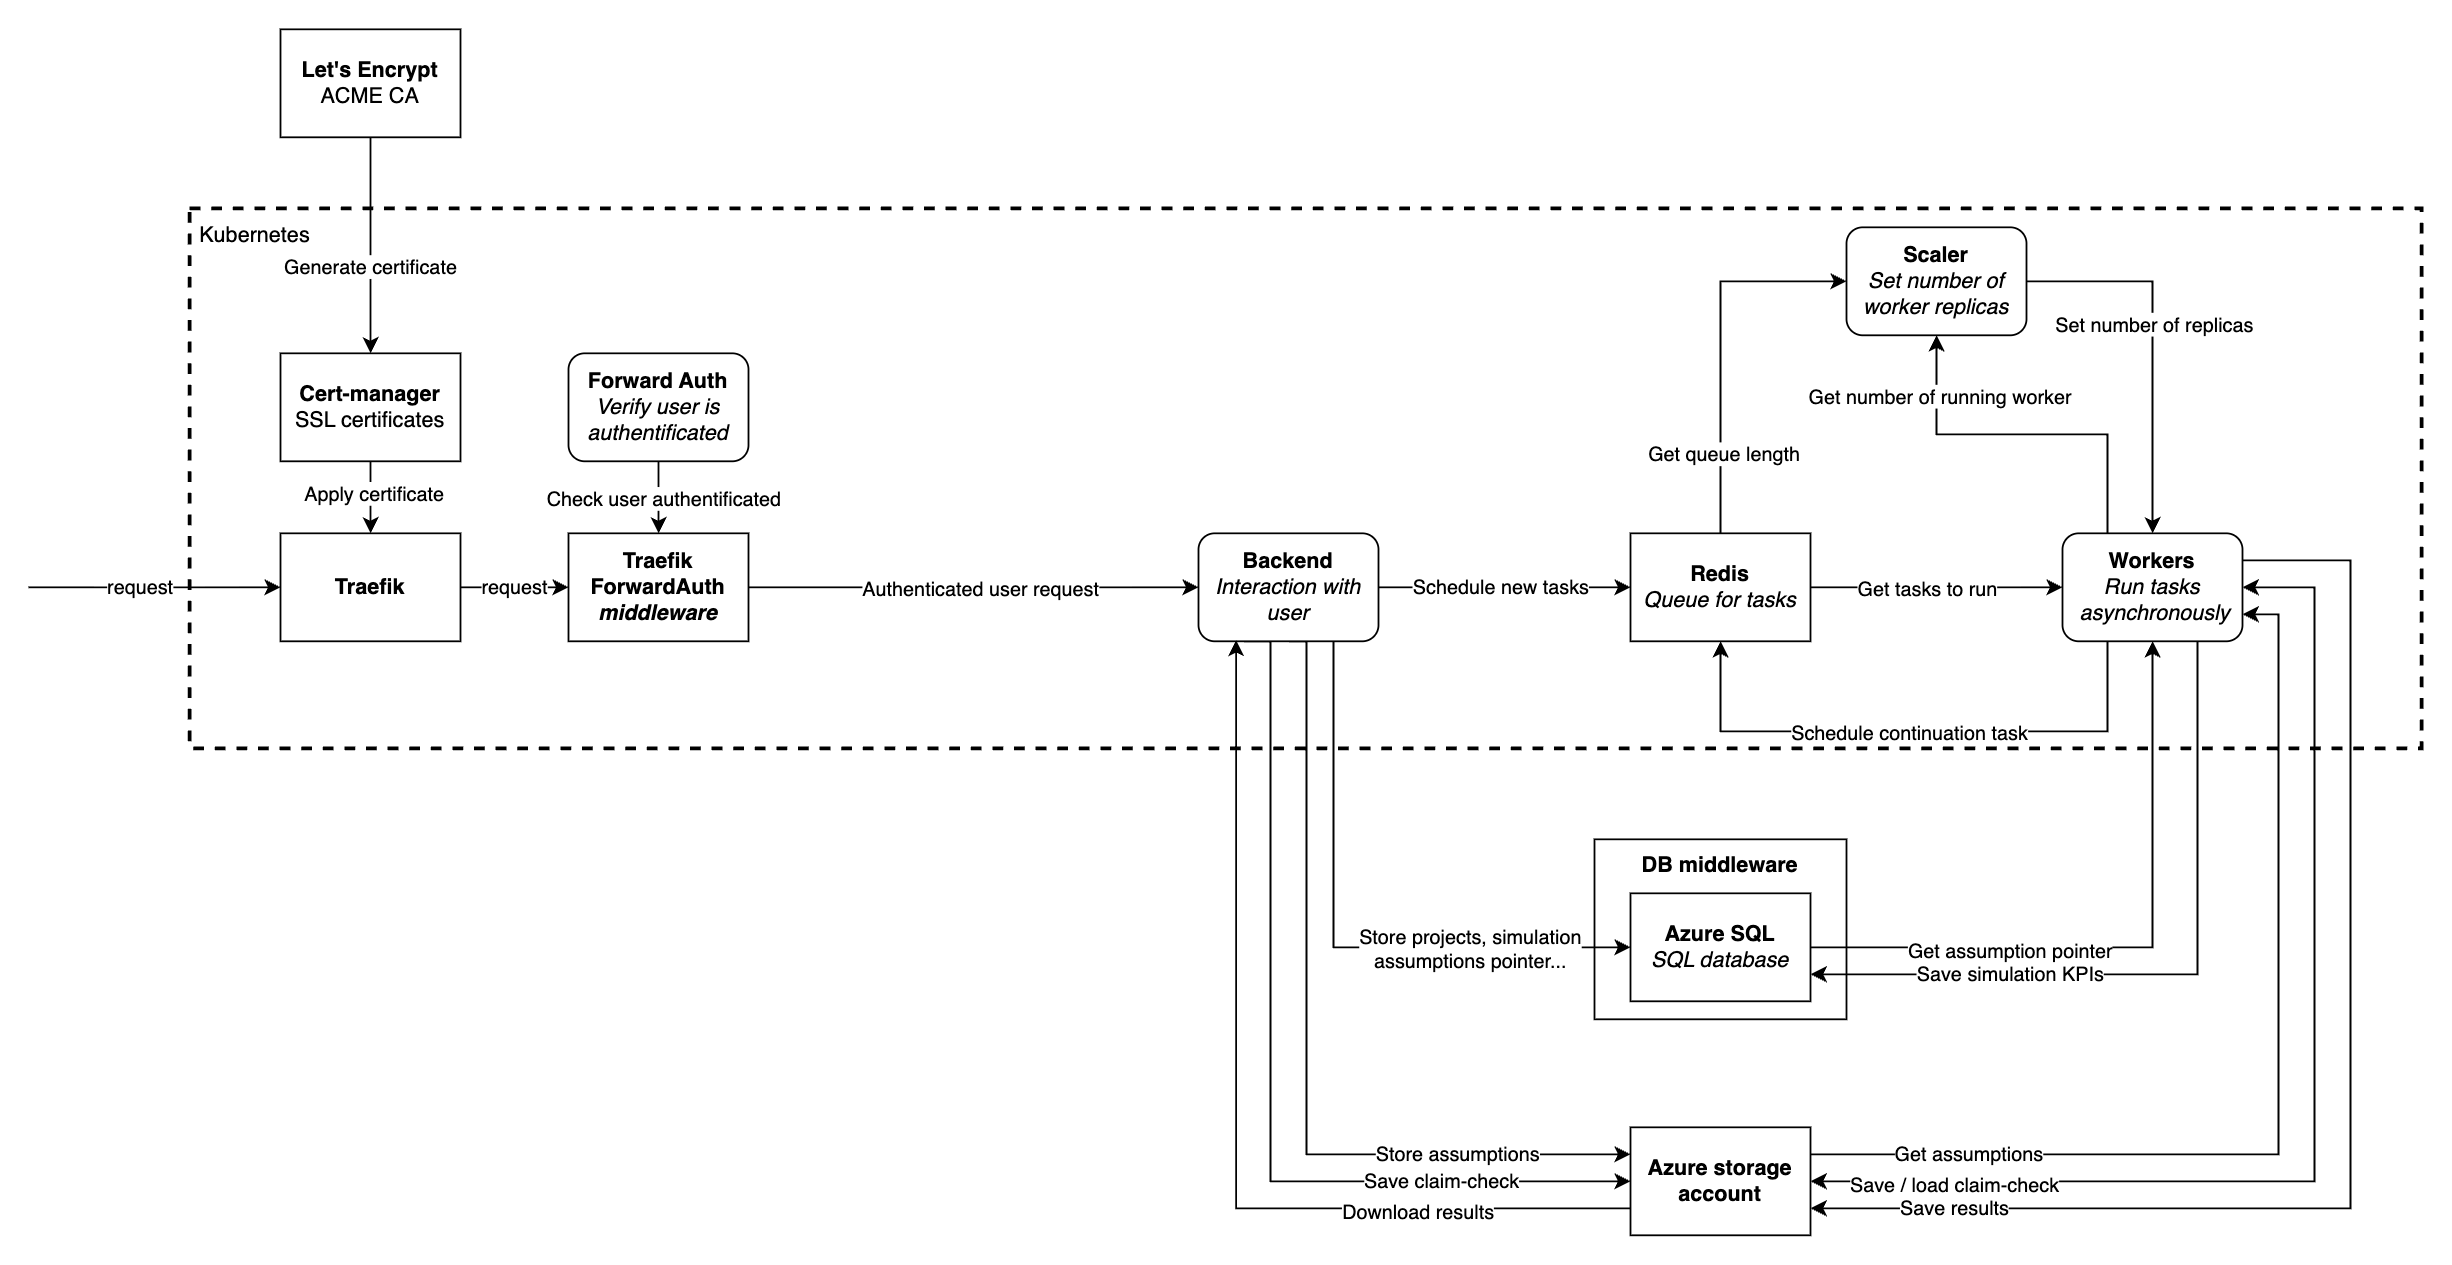
\includegraphics[width=\linewidth]{Figures/deployment_layout.png}
  \caption{Deployment on the managed Kubernetes cluster: ingress and identity edge, backend, broker, autoscaled workers, and data services.}
  \label{fig:deployment-diagram}
\end{figure}

\begin{figure}[H]
  \centering
  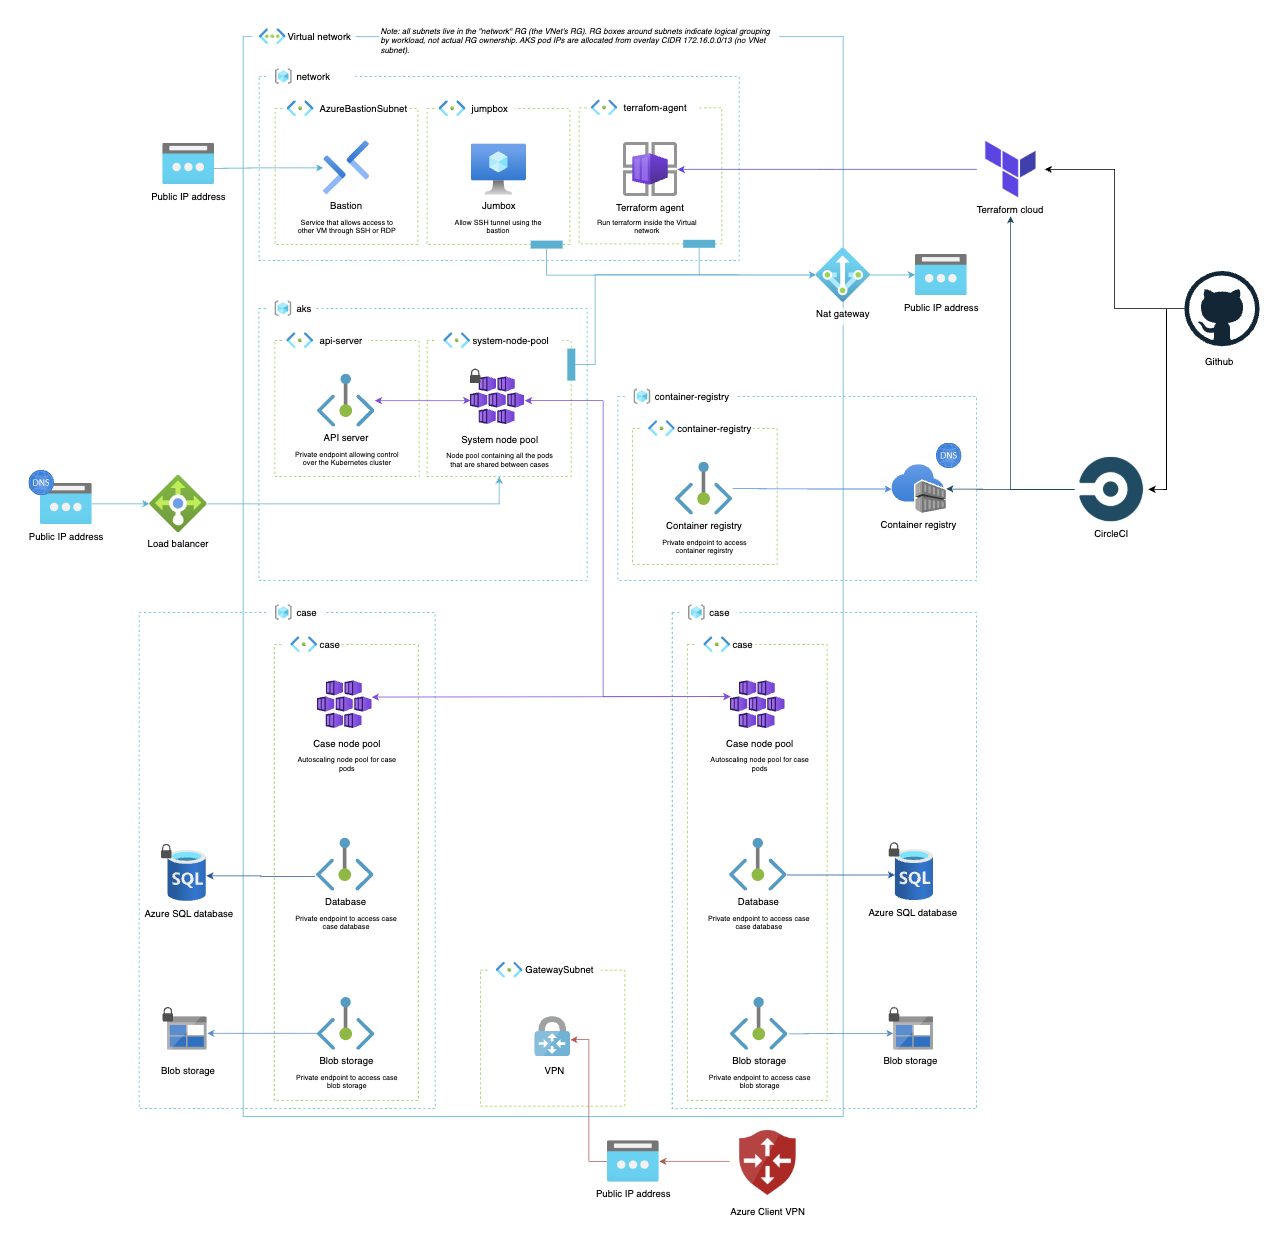
\includegraphics[width=0.82\linewidth]{Figures/azure_infrastructure.png}
  \caption{The underlying cloud infrastructure: private network, controlled admin access, managed node pools, registry, and private-endpoint data services.}
  \label{fig:azure-infra}
\end{figure}

\section{Security and trust boundaries}
\label{sec:trust}

Two trust boundaries structure the design. The first is the \textbf{platform
edge}. External users do not reach application services directly; traffic enters
through a controlled access layer that terminates secure connections and delegates
authentication to the enterprise identity provider through OpenID Connect. The
coordination layer therefore receives requests only after identity has been
established, and uses that identity to enforce access and to attribute activity to
a stable user.

This is a deliberate change from the inherited model. A security assessment of the
inherited identity layer had found weaknesses in the self-hosted setup, where
identity-provider components lived inside the application stack and had to be
patched, configured, and monitored by the product team. The chosen model delegates
sign-in to the enterprise identity provider and forwards only authenticated
traffic to the application (Table~\ref{tab:auth}), reducing the identity surface
owned by the product and aligning it with enterprise governance.

\begin{table}[H]
  \centering
  \begin{tabularx}{\linewidth}{@{}
      >{\raggedright\arraybackslash}p{3.2cm}
      >{\raggedright\arraybackslash}X
      >{\raggedright\arraybackslash}X @{}}
    \toprule
    \textbf{Aspect} & \textbf{Inherited (self-hosted)} & \textbf{Chosen (federated)} \\
    \midrule
    Identity components & Self-hosted providers inside the application stack. &
      Enterprise identity provider through OpenID Connect at the edge. \\
    \addlinespace
    Responsibility & Product team patches, configures, and monitors identity. &
      Identity lifecycle and policy handled by the enterprise. \\
    \addlinespace
    Surface & Larger security and operational surface. & Application receives only
      validated identity information. \\
    \bottomrule
  \end{tabularx}
  \caption{Shift from a self-hosted identity layer to federated enterprise
    authentication.}
  \label{tab:auth}
\end{table}

The second boundary is between \textbf{assistance and mutation}. A language model
may draft a topology change, propose assumptions, or explain results, but it must
not silently commit anything. Every state-changing operation passes through three
gates: a \textbf{typed proposal} (model output becomes a structured payload rather
than free text), \textbf{system validation} (schema, project scope, allowed
fields, and consistency with domain rules), and \textbf{human approval} (the user
explicitly accepts the action before it mutates state or launches computation).
A third boundary sits inside the platform, around the agent runtime itself: the
workers that run language-model reasoning hold no application credentials and
reach project data only through a restricted internal gateway, detailed in
Section~\ref{sec:agent-runtime}. Even if a model were manipulated into attempting
an unauthorized action, it has no direct path to the data, only the narrow,
audited path the gateway allows. The three boundaries are complementary: enterprise
identity controls \emph{who} can act, the approval discipline controls \emph{how}
assisted actions enter the authoritative system, and the runtime boundary controls
\emph{what} the reasoning workers can reach at all.

\section{Data and persistence}
\label{sec:persistence}

The product has several classes of state, and the architecture assigns each to the
storage model that fits it (Table~\ref{tab:storage}). Matching each state class to
a storage responsibility, rather than treating persistence as one undifferentiated
problem, is what keeps the system reliable as it scales.

\begin{table}[H]
  \centering
  \begin{tabularx}{\linewidth}{@{}
      >{\raggedright\arraybackslash}p{3.6cm}
      >{\raggedright\arraybackslash}X @{}}
    \toprule
    \textbf{State type} & \textbf{Storage role and reason} \\
    \midrule
    Canonical project metadata & Structured, queryable store with schema
      discipline, for consistency, auditability, and controlled evolution. \\
    \addlinespace
    Large simulation inputs and outputs & Object storage for big graph payloads,
      result files, and artifacts. \\
    \addlinespace
    Queued simulation work & Dispatch store that decouples interface
      responsiveness from execution and exposes backlog as the scaling signal. \\
    \addlinespace
    Conversational and agentic state & Durable checkpoint store so a multi-step,
      paused interaction can resume exactly where it left off. \\
    \addlinespace
    Agent run dispatch and events & Durable command, lease, and append-only event
      log owned by the agent runtime, so a run is claimed once, recovered after a
      worker loss, and its stream replayed to a reconnecting client. \\
    \addlinespace
    Observability and evaluation & Dedicated records for traces, scores, and
      feedback, kept separate from canonical project data. \\
    \bottomrule
  \end{tabularx}
  \caption{Persistence responsibilities by class of state.}
  \label{tab:storage}
\end{table}

\section{Simulation workflow architecture}
\label{sec:simworkflow}

The simulation workflow is an asynchronous pipeline
(Figure~\ref{fig:sim-sequence}). The user submits a case
through the interface; the coordination layer validates the request, records the
job, and dispatches work to the execution path; dedicated workers run the
deterministic optimization, writing outputs to durable storage; and the interface
retrieves status and results through controlled routes. Long simulations are
processed in chunks so that partial progress can be scheduled without holding the
original request open. In short, a simulation is an authenticated, queued, and
persisted workflow rather than a single blocking call, which is what makes failure
recovery explicit (through job state) rather than tied to a user session.

\begin{figure}[H]
  \centering
  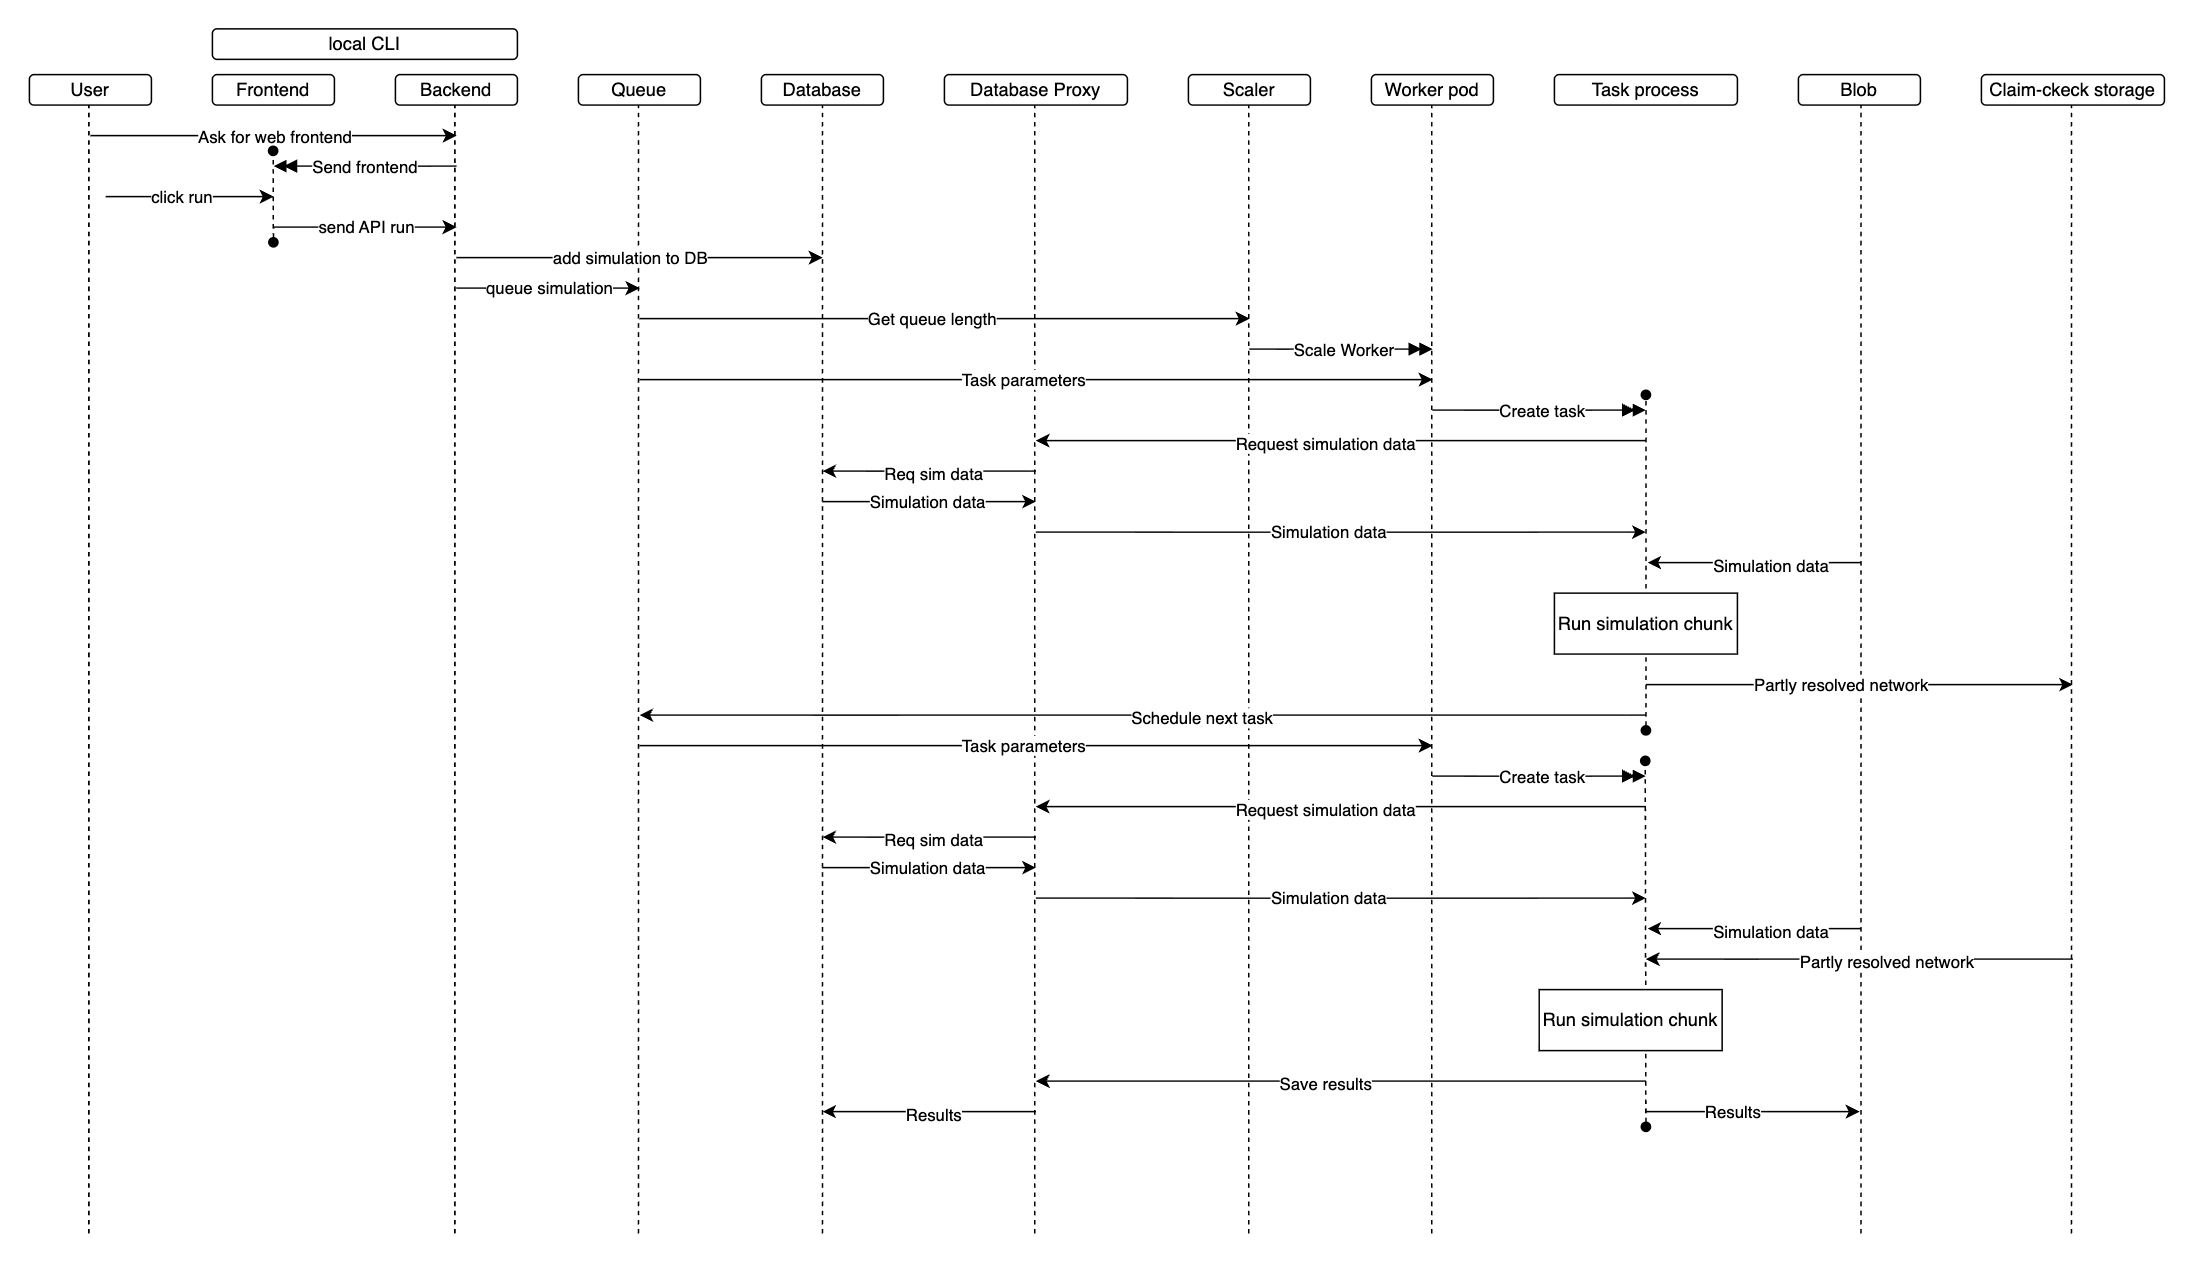
\includegraphics[width=\linewidth]{Figures/sim_sequence.png}
  \caption{End-to-end execution of a simulation run, from enqueue through autoscaled chunked execution to persisted results.}
  \label{fig:sim-sequence}
\end{figure}

A grid search adds one further concern. It can stage hundreds of scenarios at
once, and admitting them all would let a single study monopolize the workers and
would leave the results view empty until the whole sweep finished. The dispatch
path therefore applies \textbf{admission control}: it stages one queued task per
scenario but admits only a bounded number of them in flight per run, releasing the
next as running scenarios reach a terminal state. A set thus \textbf{completes
progressively}, its comparison view filling in as runs finish rather than all at
the end, and the autoscaler follows the admitted backlog rather than provisioning
for the entire sweep at once. The bound is a per-run budget, so the behavior is
inert when the budget is unlimited and adds nothing to a small study, while a large
sweep becomes usable long before it is complete.

\section{Agent runtime and durable execution}
\label{sec:agent-runtime}

The agentic layer does not run inside the application. It is a \textbf{separately
deployed runtime} with its own public boundary, its own workers, its own durable
state, and its own credentials, and the application talks to it over an internal,
versioned interface. The separation is deliberate: language-model work is
long-running, bursty, and probabilistic, so a dedicated runtime keeps its load and
its failures away from the interactive application, while keeping its access to
authoritative data narrow and auditable. This is the second execution plane of
Figure~\ref{fig:two-planes}, and it applies to agent reasoning the same discipline
the simulation plane applies to computation: durable dispatch, conditional
claiming, and checkpointed recovery.

\subsection{Service decomposition}

The runtime is decomposed into focused services with distinct credentials and
scaling (Table~\ref{tab:runtime-services}). An \textbf{Agent API} is the only
public entry point for assisted interaction; the application backend carries no
agent routes and no agent credentials. An \textbf{Agent Control} service owns
durable dispatch and the state transitions of every agent run. \textbf{Interactive}
and \textbf{heavy} worker lanes execute the reasoning graphs, the first tuned for
responsive chat turns and the second for expensive tool work, so a slow task cannot
starve a conversation. Crucially, these workers hold \textbf{no application database
or storage credentials}: every effect they need on project data passes through an
internal \textbf{Tool Gateway}, a strict boundary that exposes only a restricted,
authenticated set of operations under its own principal and is reachable solely
inside the cluster. Bulky housekeeping runs in a separate, isolated executor so
that parsing, model, gateway, and database credentials never accumulate in one
runtime closure.

\begin{table}[H]
  \centering
  \small
  \begin{tabularx}{\linewidth}{@{}>{\raggedright\arraybackslash}p{3.3cm} >{\raggedright\arraybackslash}X@{}}
    \toprule
    \textbf{Service} & \textbf{Responsibility and isolation} \\
    \midrule
    Agent API & The only public entry point for assisted interaction; creates,
      inspects, cancels, resumes, and streams runs. The backend carries no agent
      routes or credentials. \\
    \addlinespace
    Agent Control & Owns durable dispatch and every run's state transitions:
      creation, claim, progress, completion, cancellation, and recovery. \\
    \addlinespace
    Interactive workers & Execute reasoning graphs for responsive chat turns; kept
      warm so latency stays low. \\
    \addlinespace
    Heavy workers & Execute expensive tool and analysis work on a separate lane, so
      a slow task never blocks interactive turns. \\
    \addlinespace
    Tool Gateway & The strict, in-cluster boundary through which workers reach
      project data, under a restricted principal and a narrow authenticated
      interface. \\
    \addlinespace
    State and checkpoint store & Durable run records, leases, append-only events,
      and graph checkpoints, kept separate from application data. \\
    \addlinespace
    Cleanup executor & Isolated pod for bulky housekeeping, so credentials for
      parsing, models, the gateway, and the database never coexist. \\
    \bottomrule
  \end{tabularx}
  \caption{Services of the agent runtime and the isolation of each.}
  \label{tab:runtime-services}
\end{table}

\subsection{Durable dispatch, recovery, and streaming}

An agent run is not a fire-and-forget task; it is a durable command with an
explicit lifecycle (Figure~\ref{fig:agent-runtime}).

\paragraph{Durable dispatch.} When a run is created, its record and a dispatch
entry are written in a single transaction (a transactional outbox); a dispatcher
then publishes the work, and a worker \textbf{claims it conditionally} through a
lease so that exactly one worker owns a run at a time. Because message delivery is
at-least-once, every entry point is idempotent: a redelivered or already-owned run
resumes or becomes a no-op instead of duplicating work or side effects.

\paragraph{Checkpointed recovery.} Each reasoning graph is compiled with a durable
checkpointer and stable run and thread identifiers, and its work is divided at
meaningful boundaries. If a worker is lost mid-run (a deploy, an eviction, a
crash), another resumes from the last checkpoint rather than restarting or dropping
the turn. External effects are made idempotent for the same reason, since a worker
can fail after performing an effect but before recording that it did.

\paragraph{Resumable streaming.} User-visible streaming is backed by a durable
record, not only an ephemeral channel. Each run appends its events with a monotonic
per-run sequence number and then publishes them live; the Agent API replays the
persisted events after a client's cursor and continues with the live stream, so a
browser that reconnects resumes exactly where it left off, losing and duplicating
nothing. The authoritative signal is the final run status; the stream is a
replayable view of it.

\paragraph{Cancellation and bounds.} Cancellation is cooperative: a durable request
is recorded and checked between graph steps and inside long tool loops, rather than
relying on forced process termination. Each turn is bounded by a fixed execution
deadline and a per-turn context limit, so a runaway loop is stopped long before it
can exhaust a worker, and forced termination is the exception rather than the
mechanism.

\begin{figure}[H]
  \centering
  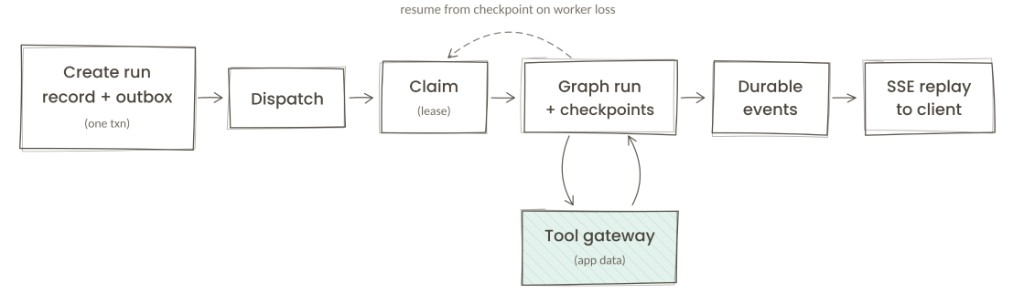
\includegraphics[width=\linewidth]{Figures/agent_runtime_flow.png}
  \caption{Lifecycle of an agent run: dispatched, claimed under a lease, executed
    as a checkpointed graph via the Tool Gateway, and streamed from a replayable
    log.}
  \label{fig:agent-runtime}
\end{figure}

The runtime scales on its own signals and is released and rolled back
independently of the application: interactive workers are kept warm for latency and
heavy workers scale with queue depth, under the same event-driven autoscaling used
for the simulation plane.

\section{The governed multi-agent layer}
\label{sec:agentic}

The agentic layer sits above the existing product as an assistant, not a
replacement. Its role is to reduce the friction of complex analytical workflows:
describing a topology, identifying missing assumptions, preparing scenario
variants, interpreting results, and guiding the user toward the next action.
Figure~\ref{fig:agentic-arch} shows the governing idea: reads execute immediately,
writes become approval-gated proposals, and the deterministic engine remains the
numerical authority.

\begin{figure}[H]
  \centering
  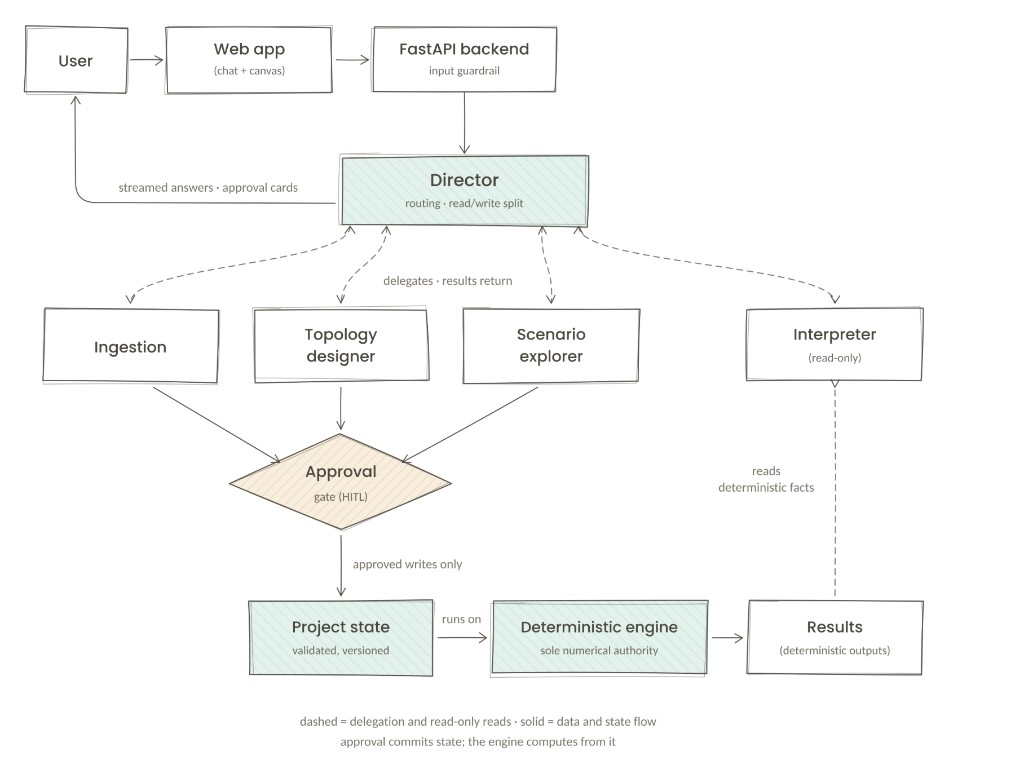
\includegraphics[width=0.92\linewidth]{Figures/agentic_flow.png}
  \caption{Governed multi-agent architecture: the Director routes each request,
    specialists propose, approved writes commit validated project state, and the
    deterministic engine computes all results (the interpreter is read-only).}
  \label{fig:agentic-arch}
\end{figure}

\subsection{Agent topology}

The agentic layer decomposes into controlled roles that form a governed hierarchy
around a single conversational entry point, rather than a set of independent
chatbots (Table~\ref{tab:agents}). The Director delegates specialist work to
focused flows, receives structured results, and turns state-changing
recommendations into approval cards. Figure~\ref{fig:agent-hierarchy}
summarizes this hierarchy and the boundary of each role.

\begin{figure}[H]
  \centering
  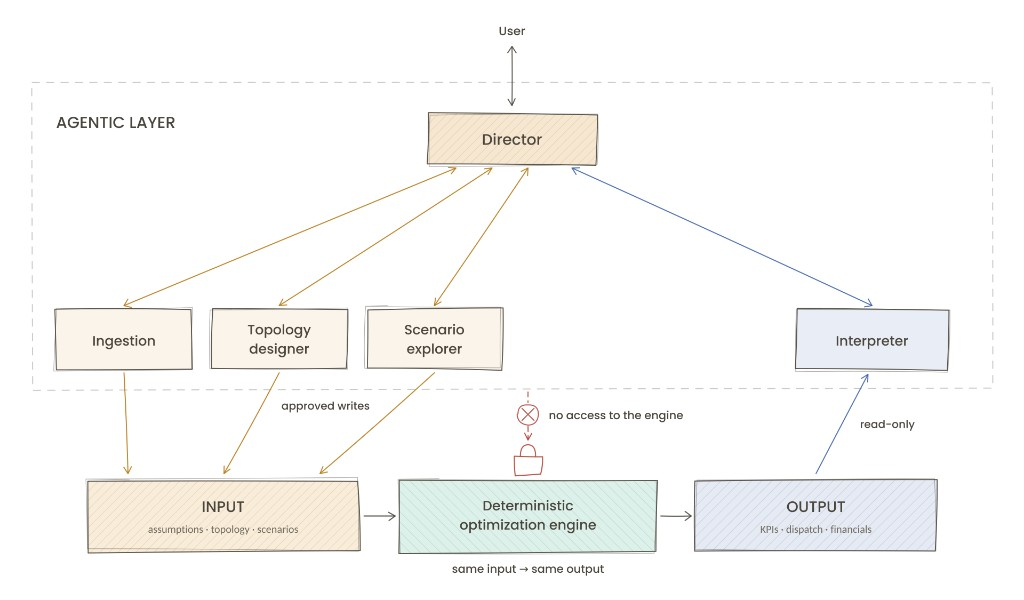
\includegraphics[width=0.95\linewidth]{Figures/agents_io_boundary.png}
  \caption{The Director and its specialists act only on the engine's inputs
    and outputs: writes are approved, reads are read-only, and the
    deterministic engine itself is never touched.}
  \label{fig:agent-hierarchy}
\end{figure}


\begin{table}[H]
  \centering
  \begin{tabularx}{\linewidth}{@{}
      >{\raggedright\arraybackslash}p{3.4cm}
      >{\raggedright\arraybackslash}X @{}}
    \toprule
    \textbf{Role family} & \textbf{Main roles and boundary} \\
    \midrule
    Conversation and approval & Director, bounded operations, proposal creation,
      pending-approval state. A single entry point: read-only operations answer
      directly, while write intent becomes an approval card before execution. \\
    \addlinespace
    Structure and ingestion & Topology Designer and Ingestion Agent. Produce draft
      topology proposals or staged assumption-file previews; project mutation
      remains approval-gated. \\
    \addlinespace
    Scenario exploration & Scenario Explorer with a scoping Analyst and four axis
      agents. Runs bounded parameter exploration and returns approval-ready canvas
      operations. \\
    \addlinespace
    Result interpretation & Interpreter agent and result-inspection
      operations. A read-only explanation loop that returns narrative and cards
      and never writes state. \\
    \bottomrule
  \end{tabularx}
  \caption{Agentic roles and their boundaries.}
  \label{tab:agents}
\end{table}

\subsection{Delegation and flow-level design}

Each flow is a controlled reasoning process with a defined state, explicit steps,
conditional routes, and local retries, rather than a single prompt. A typical turn
follows a controlled path: the Director grounds the request in the active project,
page, and conversation, answers directly or with a read-only operation when it
can, and otherwise delegates to the appropriate specialist.

\paragraph{Director.} The root reasoning flow exposed to the user. The current
message and session context enter a reason-and-act loop; the assistant either
answers or requests a bounded tool, tool results return to the reasoning path, and
the loop continues until a final answer or a proposal is emitted. Control logic
around the loop injects the active project and page, suppresses duplicate expensive
calls within a turn, and intercepts proposal-producing actions before they can be
narrated as already executed.

\paragraph{Topology designer.} A specialist flow for structural work. It resolves
the active canvas, saved topology, or previous proposal; diagnoses the task;
gathers evidence through scoped rule injection (the general rules plus the rules
for the one classified project type) and few-shot retrieval of structurally
similar library designs; generates candidate structures; compiles the chosen one
into a patch; and validates it against schema and domain rules. A design that fails
validation is not silently repaired: the flow attempts deterministic repair or
guided re-planning, and otherwise blocks with the failing evidence. Even a
successful path stores only a draft proposal.

\paragraph{Ingestion agent.} A staged, mostly deterministic pipeline that handles
uploaded assumption files as a batch. It loads the batch, parses and classifies
each file (using the model only where deterministic classification is not
confident), places recognized records into assumption slots, detects conflicts
with existing project data, stages the result, and returns a reviewable
data-quality report. The output is a preview for approval, not an immediate
mutation.

\paragraph{Scenario explorer and axis agents.} The most nested flow. A scoping
Analyst first checks that the request contains enough information (location,
activation year, plant scale, objective) and short-circuits with a clarifying
question if not. When scope is sufficient, four parallel axis agents propose sweep
values in their own domain, the technical axis for asset sizing, the commercial
axis for off-take and purchase terms, the financial axis for cost-of-capital and
tax, and the external axis for market prices and macro inputs. The Analyst
reconciles them, drops references that do not resolve against the live topology,
and returns a single validated set of canvas operations for one approval.

\subsection{Design of the result-interpretation agent}
\label{sec:interp-design}

The result-interpretation agent realizes result interpretation (F4). It explains a completed
simulation population in natural language, and its design is dominated by one
demand: it must be helpful without ever becoming a source of numerical truth.

\paragraph{A read-only reason-and-act loop.} The interpreter is not a separate
chatbot: the Director exposes it as a \textbf{single tool}, and once that tool is
called the Director suppresses its own narration for the turn, so the
interpreter's grounded voice is the only one the user hears. It runs on its
\textbf{own reasoning-capable model}, distinct from the Director's, as a small
state machine that alternates between reasoning about the user's question and
calling a read-only tool to retrieve evidence, then reasoning again over what it
retrieved, until it can answer (Figure~\ref{fig:interp-flow}). The loop is
\textbf{bounded}, by a fixed number of tool rounds and a hard timeout, so it always
terminates. Because its tools never mutate state, the interpreter needs no approval
gate, which is what allows it to answer immediately while the writing agents remain
gated.

\begin{figure}[H]
  \centering
  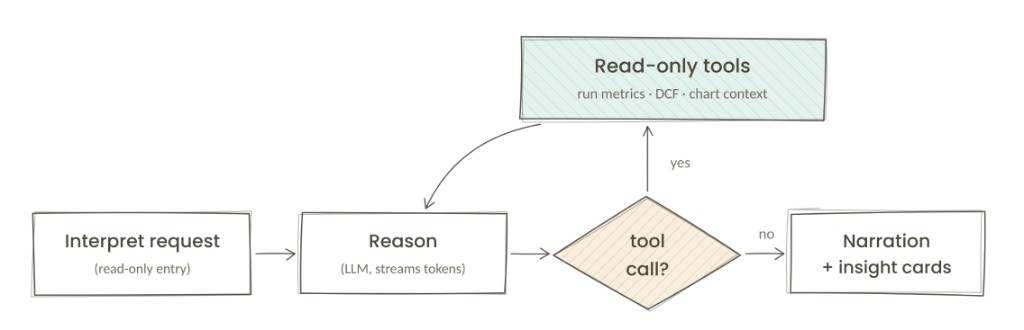
\includegraphics[width=\linewidth]{Figures/interp_flow_light.png}
  \caption{The interpreter as a read-only reason-and-act loop over deterministic
    tools, with bounded tool rounds.}
  \label{fig:interp-flow}
\end{figure}

\paragraph{Grounded, injection-resistant tool contracts.} The interpreter reasons over
facts obtained from a small set of read-only tools with structured outputs: run
metrics, discounted-cash-flow and income-statement breakdowns, sensitivities, and
chart context. The persona prompt forbids the model from computing figures itself;
every quantitative statement must cite a value returned by a tool. This is the
concrete mechanism behind the groundedness requirement (\hyperlink{nf:groundedness}{NF2}): the model organizes
and phrases evidence, but the evidence comes from the deterministic engine, so
there are no invented numbers. Decisively, these tools do not re-implement any
analysis: they call the \textbf{same pure, unit-tested functions that compute the
on-screen charts}, so the figures an explanation cites cannot differ from the
numbers the user sees.
Table~\ref{tab:interp-tools} lists the read-only tools available to the
interpreter. A useful illustration is restraint: asked to read a trend from a
scatter with a single point, the interpreter states that no relationship can be
inferred rather than fabricating one.

\begin{table}[H]
  \centering
  \small
  \begin{tabularx}{\linewidth}{@{}>{\raggedright\arraybackslash}p{4.1cm} >{\raggedright\arraybackslash}X@{}}
    \toprule
    \textbf{Read-only tool} & \textbf{What it reads} \\
    \midrule
    Result summary & The indicators available across the runs of a study. \\
    Best runs & A ranking of runs by a chosen indicator. \\
    Single-run operational read & One run's operating story (storage state, market
      trades, prices, peaks), and renders its chart. \\
    Additional chart & An extra chart panel as the narrative develops. \\
    Run configuration & The design levers of a run (asset sizes, cost of capital,
      market setup). \\
    Discounted cash flow & The per-year cash-flow table (revenue, costs, tax, net
      and cumulative flow). \\
    Scatter read & The scatter of one metric against another that the user is
      viewing. \\
    Axis-pair suggestions & Informative pairs of metrics to plot. \\
    Run comparison & The differences between two runs. \\
    Parameter suggestions & Which levers move a chosen indicator. \\
    \bottomrule
  \end{tabularx}
  \caption{The interpreter's read-only tools, each returning facts from the same analytics that produce the charts.}
  \label{tab:interp-tools}
\end{table}

\paragraph{Streaming and bounded turns.} The interpreter streams its narration
token by token so that the user receives feedback immediately, and returns a set of
\textbf{insight cards} alongside the prose, optionally embedding the chart the
explanation refers to. Each interpretation runs as a \textbf{fresh, stateless
turn}: no prior conversation enters it, only the analyst persona and the on-screen
question, and only compact, pre-aggregated facts reach the model, each truncated to
a hard ceiling. The turn therefore stays small by construction and never approaches
the context limit, which keeps it fast and cheap as well as grounded.

\subsection{Graph control principles}

Across all these flows, the same control principles apply: \textbf{typed state}
(each flow carries an explicit schema), \textbf{conditional routing} (blocking
conditions, missing inputs, and repair paths are explicit routes),
\textbf{local retries} (transient or malformed outputs are retried inside the flow
that owns the failure), \textbf{progress streaming} (long flows emit progress
events so the interface can show which lane is running), and \textbf{deterministic
final authority} (even a successful assisted flow only prepares inputs or scenario
definitions). The approval gate (F6) is thus part of the architecture, not a
user-interface detail: the model may recommend, the system validates, the user
approves, and only then may state change.

\section{Design of the visualization layer}
\label{sec:viz-design}

The visualization layer realizes results visualization (F5) and is the
surface on which interpretation is offered. It is built as a set of components over
the deterministic outputs, organized so that a user moves naturally from comparing
a whole population of runs, to reading one run in depth, to asking for an
explanation of exactly what is on screen.

\paragraph{Two views.} The results are presented through two tabs. A
\textbf{library} view manages the runs of the
selected studies: it lists every
simulation with its live status, supports search, download, and cancellation, and
refreshes while work is still in progress. A \textbf{chart} view is the analytical
core, laid out top to bottom as controls, a comparison scatter, and a per-run
dashboard. The realized views are shown in Chapter~\ref{chap:implementation}
(Figures~\ref{fig:impl-library} and~\ref{fig:impl-scatter}).

\paragraph{Comparing runs: the scatter.} The central element is a \textbf{scatter
with selectable axes}: one point per simulation
across the selected studies,
positioned by any pair of financial or operational indicators, which makes
trade-offs (for example capital cost against return) and standout runs immediately
visible. The axis choices are not a flat list. They are grouped into scanned
inputs, indicator outputs, constant quantities, and pairs that are incompatible
with the current axis, and a pair is offered only when the two metrics actually
share data across the selected runs, which prevents empty or degenerate plots.
Hovering a point reveals its key metrics and asset configuration; clicking it
selects the run and opens its dashboard; and a box drawn on the plot zooms into a
region, with each study drawn in its own marker and color so several sets can be
compared at once.

\paragraph{Reading one run: the operational dashboard.} Selecting a point opens a
dashboard that tells that run's \textbf{operational money story} across six panels
(Table~\ref{tab:viz-panels}; realized in
Figure~\ref{fig:impl-dashboard}), governed by a time-filter sidebar that sets the scope
and granularity, from a monthly overview down to a scoped hourly window. Panels
appear only for the assets a run actually contains, so an islanded plant or a plant
without storage simply omits the panels that do not apply.


\begin{table}[H]
  \centering
  \small
  \begin{tabularx}{\linewidth}{@{}>{\raggedright\arraybackslash}p{4.2cm} >{\raggedright\arraybackslash}X@{}}
    \toprule
    \textbf{Panel} & \textbf{What it shows} \\
    \midrule
    Effective revenue & Revenue over time, with cumulative revenue on a second
      axis. \\
    Market imports and exports & Quantity bought and sold per market over time, with
      price on a second axis; a market picker and quantity, revenue, or price
      modes. \\
    Energy mix & Generation over time by source, for the sources present in the
      topology. \\
    Battery state of charge & When the battery charges and discharges over time. \\
    Solar load factor & Average solar utilization over time. \\
    Wind load factor & Average wind utilization over time. \\
    \bottomrule
  \end{tabularx}
  \caption{The per-run operational dashboard: the six panels of a run's operational money story.}
  \label{tab:viz-panels}
\end{table}

\paragraph{The financial view.} Alongside the operational panels, a dedicated
component renders the \textbf{discounted-cash-flow and income statement} as a
grouped, expandable table (years by line items) with drill-down to per-asset and
per-market components, amortization and debt groups, reconciliation, payback
highlighting, sign-aware formatting, and hover-for-exact-figure
(Figure~\ref{fig:viz-financial}). It turns a dense
financial statement into something a non-specialist can navigate and audit.

\begin{figure}[H]
  \centering
  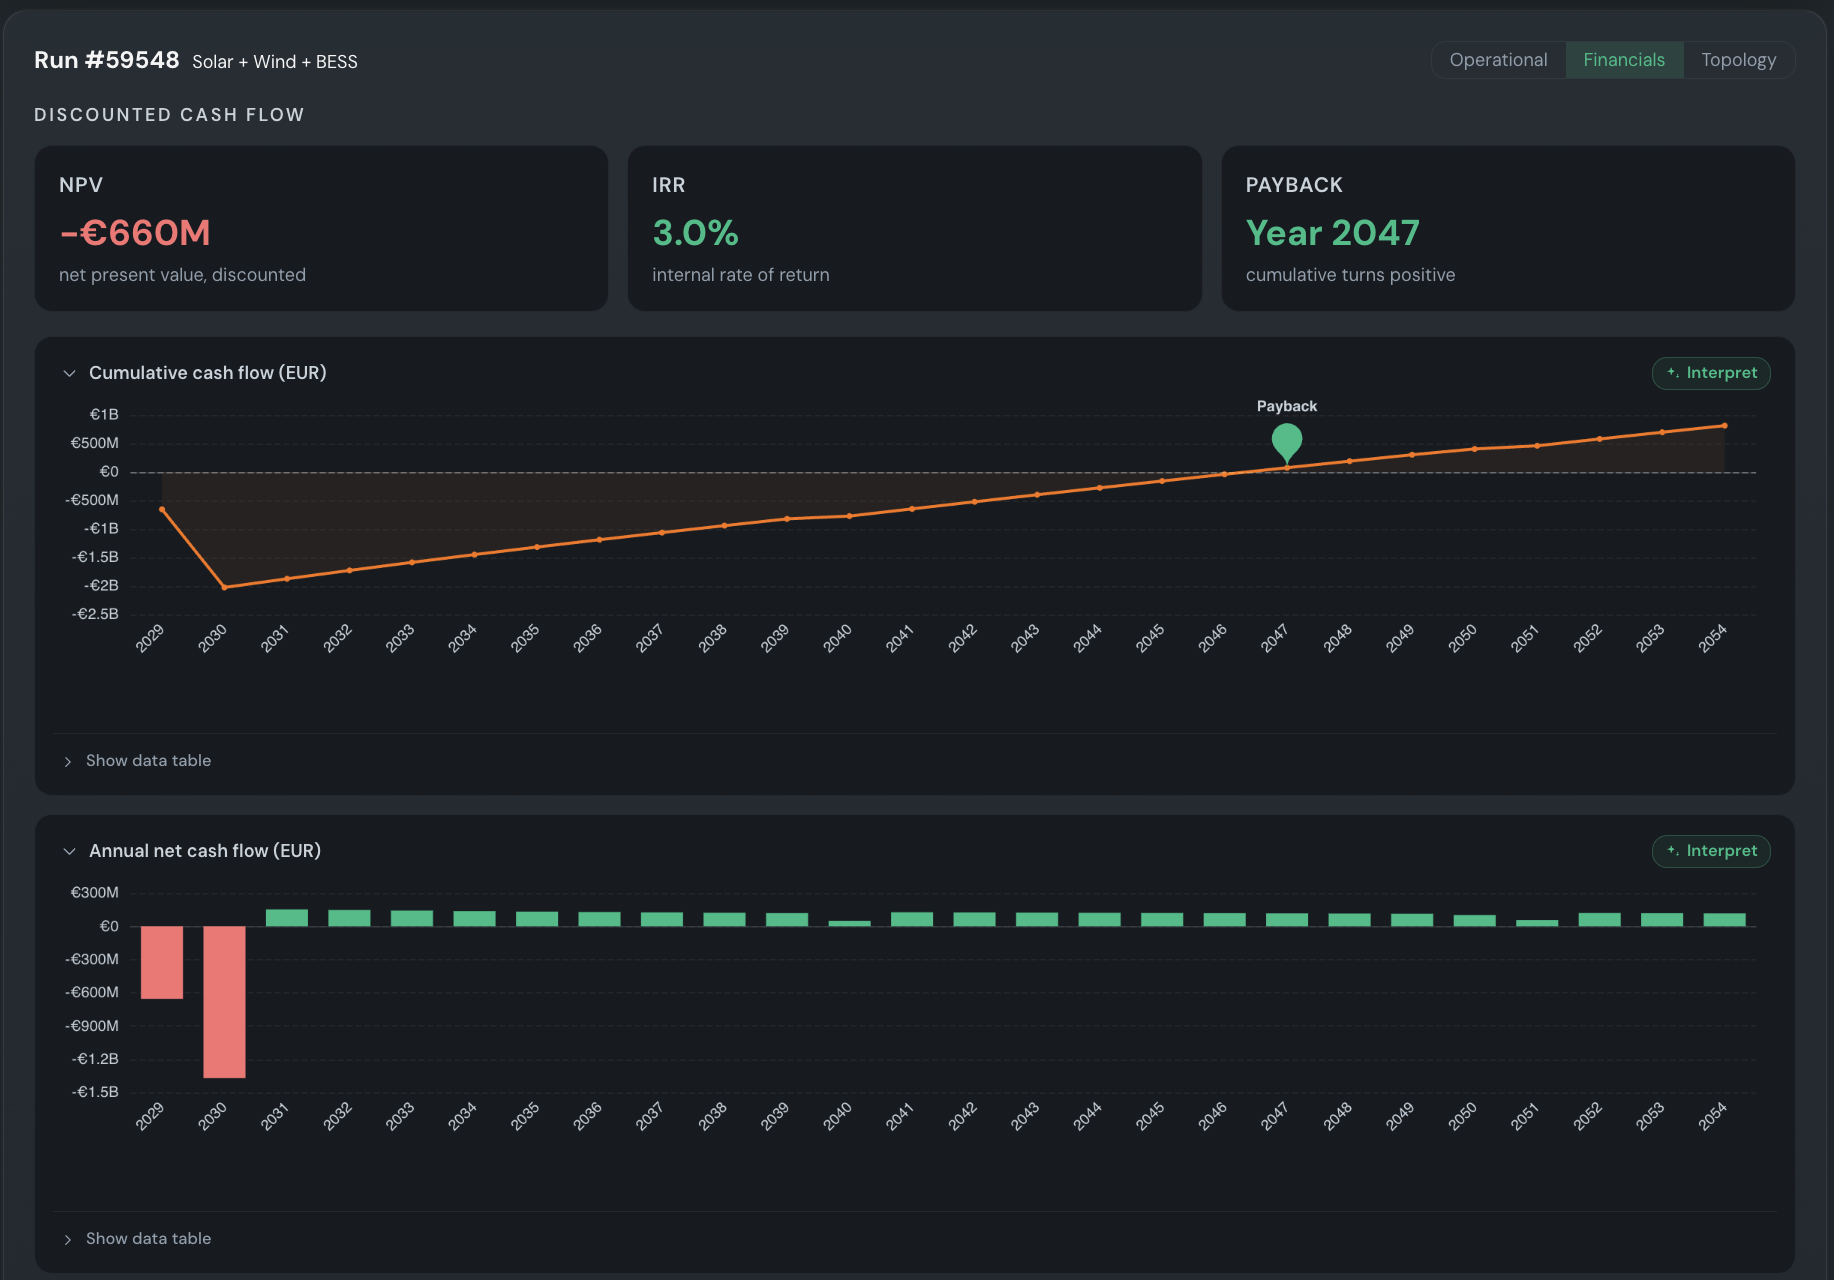
\includegraphics[width=0.8\linewidth]{Figures/05.png}
  \caption{The financial view of a run: headline indicators (NPV, IRR, payback)
    above the cumulative and annual discounted-cash-flow charts.}
  \label{fig:viz-financial}
\end{figure}

\paragraph{Interpret on demand.} Finally, each chart exposes an
\textbf{interpret-on-demand} action that attaches a grounded, streamed explanation
from the interpreter to the exact view the user is looking at, passing along the
run, the time window, the granularity, and any active filters. Because both the
charts and the interpreter read the same deterministic analytics, the figures the
explanation cites cannot differ from the figures the chart plots. This ties
visualization and interpretation
together while keeping the boundary between shown data and generated commentary
clear; the realized interface is shown in Chapter~\ref{chap:implementation}
(Figure~\ref{fig:impl-interp}).

\section{Design of the evaluation harness}
\label{sec:eval-design}

Because the assisted capabilities rely on a language model, their quality has to be
measured rather than assumed (\hyperlink{nf:eval}{NF6}). The evaluation harness
(F7) turns that requirement into a concrete mechanism.

\paragraph{An independent judge.} Interpretations are free text, so they are scored
by an independent \textbf{judge model} on four dimensions, each from 0 to 1
(Table~\ref{tab:judge}), against a rubric distilled from the product's own
financial and commercial expert prompts, so the grading reflects real domain rules.
The judge is a single call made \emph{outside} the interpreter loop: a grading
hiccup can therefore never break the user's answer, and an independent grader is
more trustworthy than a model grading itself. Each case is scored more than once and
aggregated, since a single judgement is noisy. The four scores as they appear on a
real trace are shown in Chapter~\ref{chap:implementation}
(Figure~\ref{fig:impl-judge-scores}).

\begin{table}[H]
  \centering
  \small
  \begin{tabularx}{\linewidth}{@{}>{\raggedright\arraybackslash}p{3.7cm} >{\raggedright\arraybackslash}X@{}}
    \toprule
    \textbf{Dimension} & \textbf{What it checks} \\
    \midrule
    Groundedness & Every figure traces back to a tool fact, with no invented
      numbers. The most checkable and most trustworthy dimension. \\
    Financial soundness & Cost-of-capital and discounting use, cash-flow
      consistency, depreciation and tax, currency consistency. \\
    Commercial soundness & Realistic price bands for the market setup; an islanded
      plant treated differently from a traded one. \\
    Operational coherence & A causal charge, discharge, and market story that
      actually hangs together. \\
    \bottomrule
  \end{tabularx}
  \caption{The rubric the judge scores each interpretation against.}
  \label{tab:judge}
\end{table}

\paragraph{Online and offline.} The same judge runs in two modes. \textbf{Online},
after each interpretation it fires in the background (sampled, so cost can be dialed
down) and writes the four scores onto that turn's trace, which makes quality visible
live without delaying the user. \textbf{Offline}, it runs over a curated dataset
through a harness, so a change to the interpreter's prompt or the expert rubrics is
validated by re-running and comparing the score deltas across versions on the same
cases.



\paragraph{A closing feedback loop.} Users rate each answer with a thumbs signal
that is recorded as a score; nightly jobs promote weak turns into the review
dataset and re-run the evaluation. Poor answers are thus surfaced and become the
next round of prompt work, so the system does not only explain results, it
\textbf{measures and improves its own explanations} over time
(Figure~\ref{fig:eval-loop}).

\paragraph{Structural fidelity.} A complementary method covers the components that
produce a graph, notably the topology designer: fidelity is measured against
curated golden references using the graph edit distance, which captures structural
similarity that string comparison cannot. Together, the free-text judge and the
structural metric cover both kinds of assisted output the platform produces.

\begin{figure}[H]
  \centering
  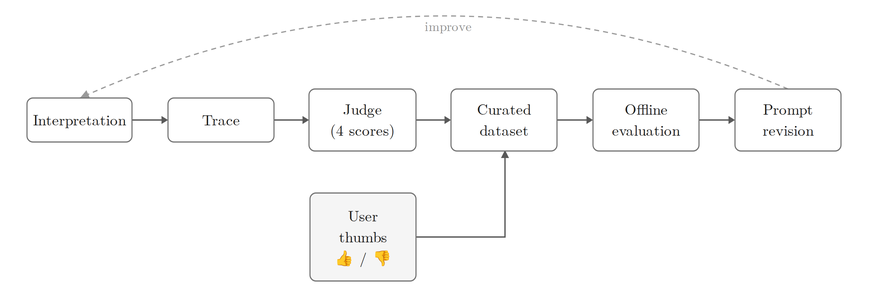
\includegraphics[width=\linewidth]{Figures/11.png}
  \caption{The evaluation loop: each interpretation is traced and judged on four dimensions, with weak turns re-scored offline.}
  \label{fig:eval-loop}
\end{figure}

\section{Interaction design}
\label{sec:interaction}

The interface must support two kinds of work: conventional analytical workflows
(project navigation, topology editing, scenario configuration, result exploration)
and conversational assistance (streamed responses, proposal cards, approval and
rejection controls, and validation feedback). It is therefore treated as a coherent
design system rather than a collection of unrelated screens: the same primitives,
buttons, forms, tables, dialogs, status badges, and cards, behave consistently
whether the user is editing manually or responding to an assistant proposal. This
consistency is also a trust decision, because it lets users reliably distinguish
draft, pending, approved, and committed states, which makes the governance of the
agentic layer visible rather than hidden.

\section{Observability and operational architecture}
\label{sec:observability}

The architecture requires operational controls around the runtime, split between
the application layer and the platform layer. Observability records every model
call, tool invocation, latency, cost, and evaluator score, so that a visible answer
can be traced back to the exact reasoning and evidence that produced it, and so
that assisted behavior can be debugged and costed. Because the agent runtime is a
separate service, a single trace is propagated across the boundary, from the
application request through the Agent API, the worker, the reasoning graph, and its
model and tool calls, so that even a cross-service answer can be followed end to
end.

Beyond tracing, the platform includes an \textbf{operational monitoring loop}
around a \textbf{read-only assessment agent}. On a schedule, a runner performs
deterministic health checks first, public and internal reachability, read-only API
checks, and a synthetic end-to-end journey in a temporary test project, and then
asks the read-only assessment agent for an evidence-based status. The agent can
inspect resources, logs, traces, and route health, but its toolset excludes any
mutation; the runner, not the agent, owns the few bounded side effects (creating
and deleting the synthetic test project, storing the report, and sending
notifications). The output is a compact status, GREEN, YELLOW, or RED, with
evidence and suspected causes; the delivered report is shown in
Chapter~\ref{chap:implementation} (Figure~\ref{fig:impl-qa}). Keeping the
assessment agent read-only mirrors, at
the platform level, the same assistance-versus-authority principle that governs the
product agents.

\section{Architecture summary}
\label{sec:arch-summary}

Table~\ref{tab:responsibilities} summarizes the responsibilities and trust
principle of each layer. The deterministic core remains authoritative; the platform
makes it secure and deployable; the interaction layer makes it usable; the execution
and persistence design make it scalable; observability and monitoring make its
behavior inspectable; and the agentic layer makes complex workflows easier without
weakening auditability.

\begin{table}[!ht]
  \centering
  \begin{tabularx}{\linewidth}{@{}
      >{\raggedright\arraybackslash}p{3.1cm}
      >{\raggedright\arraybackslash}X
      >{\raggedright\arraybackslash}p{4.2cm} @{}}
    \toprule
    \textbf{Layer} & \textbf{Primary responsibility} & \textbf{Trust principle} \\
    \midrule
    Presentation & Make project, topology, scenario, result, and approval
      workflows usable. & Show state clearly; never hide proposed mutations. \\
    \addlinespace
    Coordination & Validate requests, serve state, coordinate persistence and
      dispatch. & Centralize state transitions behind typed contracts. \\
    \addlinespace
    Deterministic execution & Run optimization workloads and produce auditable
      numerical outputs. & Keep computation reproducible and independent of the
      language model. \\
    \addlinespace
    Persistence & Store canonical data, large artifacts, dispatch state, and
      checkpoints. & Match storage to state type and recovery need. \\
    \addlinespace
    Agent runtime & Assist through routing, specialists, and interpretation, on a
      separate, durably dispatched execution plane. & Hold no direct data access;
      propose under constraints; mutate only after validation and approval. \\
    \addlinespace
    Platform & Provide managed runtime, authenticated access, and observability. &
      Make delivery repeatable, auditable, and enterprise-aligned. \\
    \bottomrule
  \end{tabularx}
  \caption{System responsibilities and trust principles by layer.}
  \label{tab:responsibilities}
\end{table}

\section*{Conclusion}

This chapter presented the full architecture around the deterministic core: the
architectural objectives, the logical decomposition and its graph views, the
runtime and cloud deployment model, the security and identity boundaries, the
persistence and simulation workflow, and the governed multi-agent layer with each
of its agents. It detailed the design of the read-only interpreter, the
visualization layer, and the evaluation harness within that complete system, and
it showed how every layer
upholds the principle that assistance never becomes numerical authority. The next
chapter turns this design into a concrete implementation and reports its
evaluation.
